\documentclass{beamer}
\usetheme{MinimalGreen/beamerthemeMinimalGreen}
\usepackage{hyperref}
\usepackage[utf8]{inputenc} % this is needed for german umlauts
\usepackage[english]{babel} % this is needed for german umlauts
\usepackage[T1]{fontenc}    % this is needed for correct output 
                            % of umlauts in pdf
\usepackage{graphicx}
\usepackage{braket}

\begin{document}

\title{Spin Networks for Perfect State Transfer}
\author{dln-dev}
\date{5. April 2016}

\frame{\titlepage}

\section{Introduction}
\subsection{Motivation}
\begin{frame}{Hardware}
	\begin{columns}[T]
		\begin{column}{0.33\textwidth}
			\centering
   			Processors
   			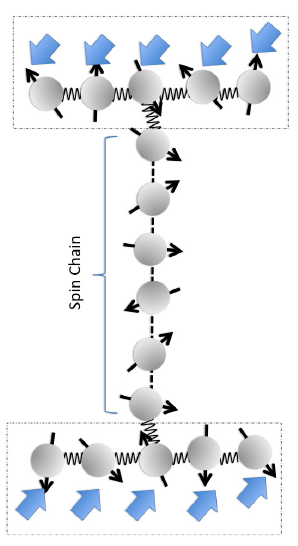
\includegraphics[width=\textwidth]{Images/processor}
		\end{column}
		\uncover<2->{\begin{column}{0.33\textwidth}
			\centering
    		Computers
    		\includegraphics[trim=0 0 0 -40mm, width=\textwidth]{Images/computer}
		\end{column}}
     	\uncover<3->{\begin{column}{0.33\textwidth}
     		\centering
     		Computing
     		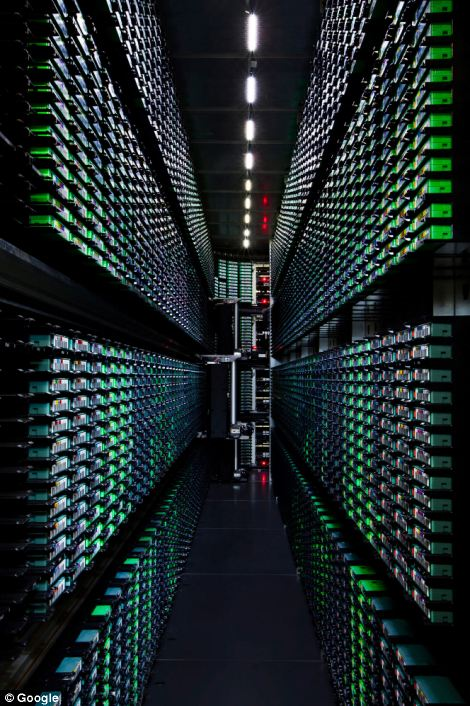
\includegraphics[trim=0 0 0 -20mm, width=\textwidth]{Images/computing}
		\end{column}}
	\end{columns}
\end{frame}

\subsection{Requirements}
\begin{frame}{Requirements}
	\begin{itemize}
		\item Separation of highly controlled regions
		\item Spacers
		\begin{itemize}
			\item (Perfect) state transfer
			\item Fixed interactions
			\item Natural dynamics
			\item Control over single qubit at each end only (for now)
		\end{itemize}
	\end{itemize}
	
	$\rightarrow$ Spin networks!
%Registers are highly controlled regions (gates, ...), probably need separation, spacers need to be capable of state transfer -> spins, control free region: permanent, fixed interactions between spins, natural dynamics (initialize, wait, read); For now: only single qubits control at each site, homogenous constant couplings, PST (Explain!), spin networks instead so no transformation is needed.
\end{frame}

\subsection{Model}
\begin{frame}[t]{Model}	
	\begin{exampleblock}{}
	\setlength\abovedisplayskip{-8pt}
	\begin{center}
		\[H_{XX}=\frac{1}{2}J\sum_{i=1}^{N}{\left[\sigma_i^x\sigma_{i+1}^x + \sigma_i^y\sigma_{i+1}^y\right]}\]
	\end{center}
	\end{exampleblock}
	\begin{itemize}
		\item $J\equiv const.$
		\item No z coupling
		\item $\left[H_{XX},\sigma^z_\text{tot}\right] = 0$
		\item Eigenstates: $ $
		\item Eigenvalues: $ $
	\end{itemize}
%    Show complete Heisenberg model (no local potentials), explain terms, why no z coupling etc., commutes with total z spin, then XY model, what do states look like?
\end{frame}

\subsection{Math setup}
\begin{frame}{Math setup}
	\begin{description}
	\item [Ground state of ferromagnetic spin-$\frac{1}{2}$ chain:] \[ \ket{\uparrow}_1 \otimes \ket{\uparrow}_2 \otimes \dots \otimes \ket{\uparrow}_N = \ket{\uparrow_1\uparrow_2\dots\uparrow_N} := \ket{0} \]
	\item [Excitation operator $\sigma^- = \frac{1}{2}\left(\sigma^x - \text{i}\sigma^y\right)$:] \[ \text{1}_1 \otimes \text{1}_2 \otimes \dots \otimes \text{1}_{j-1} \otimes \sigma^- \otimes \text{1}_{j+1} \otimes \dots \otimes \text{1}_N := \sigma^-_j \]
	\item [Single spin excitation:] \[ \sigma^-_j\ket{0} := \ket{j} \]
	\item [Single spin superposition:] Prepare $j$th spin as $\alpha\ket{\uparrow}_j + \beta\ket{\downarrow}_j \rightarrow$ \[ \ket{\Psi} := \alpha\ket{0} + \beta\ket{j} \]
	\end{description}
%    Explain numbers as kets, superpositions, graphs, later binary scheme for graphs, adjacency matrices and correspondence to hamiltonian, fidelity.
\end{frame}

\begin{frame}{Perfect state transfer}
	In general, target state will evolve into a mixed state:\\
	\[ \rho_{out} = P(t)\ket{\Psi_{out}}\bra{\Psi_{out}} + \left( 1-P(t) \right)\ket{\uparrow}\bra{\uparrow} \]
	with
	\[ \ket{\Psi_{out}} = \frac{1}{\sqrt{P(t)}}\left( \cos{\left(\frac{\Theta}{2}\right)} \ket{\uparrow} + e^{\text{i}\Phi}\sin{\left(\frac{\Theta}{2}\right)}f^N_{r,s}(t)\ket{\downarrow} \right) \]
%	and
%	\[ P(t) = \cos^2{\left(\frac{\Theta}{2}\right)} + \sin^2{\left(\frac{\Theta}{2}\right)}\lvert f^N_{r,s}(t)\rvert^2 \]
	Transition amplitude: $f^N_{r,s}(t) = \bra{r}e^{\text{i}H t}\ket{s}$\\
	\begin{exampleblock}{}
	\setlength\abovedisplayskip{-8pt}
	\begin{center}
		\[ \text{Fidelity:}\mathfrak{F}(t) = \frac{1}{4\pi}\int \!\bra{\Psi_{in}}\rho_{out}\ket{\Psi_{in}} \, \mathrm{d}\Omega = \frac{\lvert f^N_{r,s}\rvert\cos{\lambda}}{3} + \frac{\lvert f^N_{r,s}\rvert^2}{6} + \frac{1}{2}\]
% in order to give qualitative statements it suffices to know f^N_r,s
	\end{center}
	\end{exampleblock}
\end{frame}

\begin{frame}[t]{Graphs}
	\begin{exampleblock}{}
	\setlength\abovedisplayskip{-8pt}
	\begin{center}
		$G = (V,E)$
	\end{center}
	\end{exampleblock}
	\begin{itemize}
		\item Edges undirected $\rightarrow E \subseteq \{\{i,j\}\colon i,j \in V\}$
		\item Single edges only $\rightarrow \{i,j\}$ unique
	\end{itemize}   
%	is a subset of the set of all unordered pairs of vertices in $V$.
	Example: $V = \{1,2,3\}, E = \{\{1,2\},\{2,3\}\}$
\end{frame}

\begin{frame}[t]{Adjacency Matrices}
	\begin{exampleblock}{}
	\setlength\abovedisplayskip{-8pt}
	\begin{center}
		$a_{ij} = \left\{
	\begin{array}{ll}
		1  & \{i,j\} \in E \\
		0  & \text{otherwise}
	\end{array}
\right.$	
	\end{center}
	\end{exampleblock}
	\begin{itemize}
		\item No multi-edges $\rightarrow$ all elements either $0$ or $1$
		\item Unordered Pairs $\rightarrow$ symmetric
		\item Orthogonal basis exists, eigenvalues are roots of $det(A-\lambda \text{1}) = 0$
	\end{itemize}
	\begin{columns}[T]
		\begin{column}{0.5\textwidth}
			\centering
   			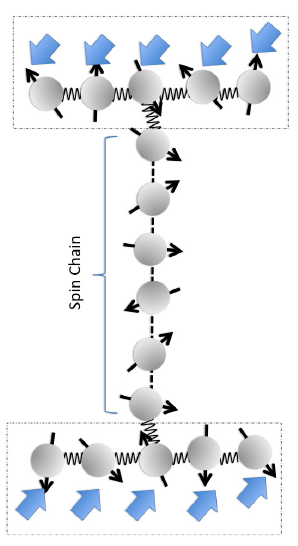
\includegraphics[width=\textwidth]{Images/processor}
		\end{column}
		\begin{column}{0.5\textwidth}
			\centering
    		\includegraphics[trim=0 0 0 -40mm, width=\textwidth]{Images/computer}
		\end{column}
	\end{columns}
\end{frame}

\begin{frame}{Correspondence to Hamiltonians}
	\begin{columns}[T]
		\begin{column}{0.33\textwidth}
			\centering
   			4-qubit chain
   			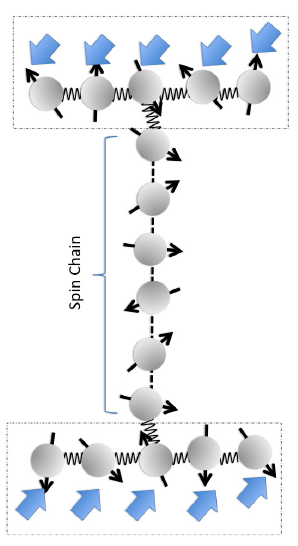
\includegraphics[width=\textwidth]{Images/processor}
		\end{column}
		\uncover<2->{\begin{column}{0.33\textwidth}
			\centering
    		6-qubit ring
    		\includegraphics[trim=0 0 0 -40mm, width=\textwidth]{Images/computer}
		\end{column}}
     	\uncover<3->{\begin{column}{0.33\textwidth}
     		\centering
     		Single spin subspace
     		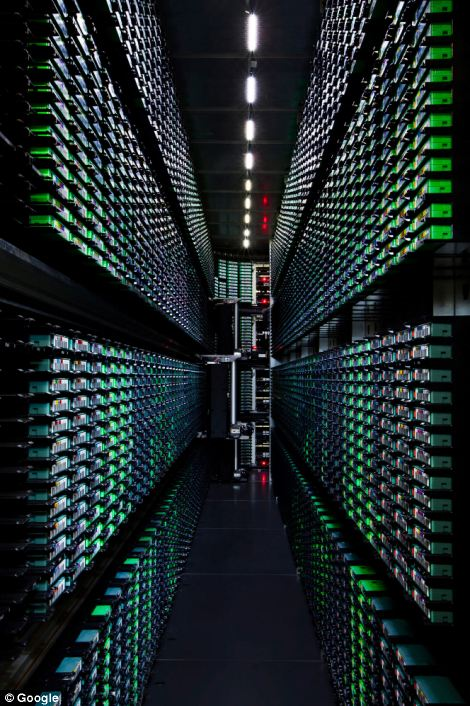
\includegraphics[trim=0 0 0 -20mm, width=\textwidth]{Images/computing}
		\end{column}}
	\end{columns}
\end{frame}

\begin{frame}[t]{Cartesian Product of Graphs}
	\begin{exampleblock}{}
	\setlength\abovedisplayskip{-8pt}
	\begin{center}
		$G \times H = (V_{G\times H},E_{G\times H})$
	\end{center}
	\end{exampleblock}
	\begin{itemize}
		\item $V_{G\times H} = V(G) \times V(H)$
		\item $\{(u,u'),(v,v')\} \in E_{G\times H}$ if 
		\begin{itemize}
			\item $u = v$ and $\{u',v'\} \in E_H$ or
			\item $u' = v'$ and $\{u,v\} \in E_G$
		\end{itemize}
	\end{itemize}
	\begin{exampleblock}{}
	\setlength\abovedisplayskip{-8pt}
	\begin{center}
		$A_{G\times H} = A_G \otimes \text{1}_{(V_H)} + \text{1}_{(V_G)} \otimes A_H$
	\end{center}
	\end{exampleblock}
\end{frame}

\begin{frame}{Examples of Product Graphs}
	\begin{columns}[T]
		\begin{column}{0.33\textwidth}
			\centering
   			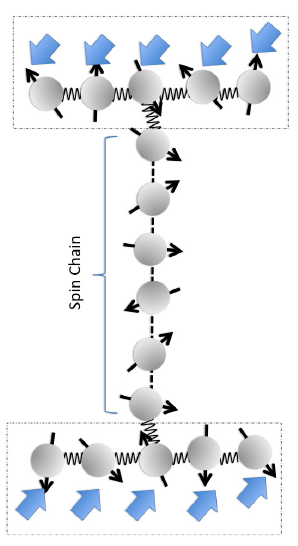
\includegraphics[width=\textwidth]{Images/processor}
		\end{column}
		\uncover<2->{\begin{column}{0.33\textwidth}
			\centering
    		\includegraphics[trim=0 0 0 -40mm, width=\textwidth]{Images/computer}
		\end{column}}
     	\uncover<3->{\begin{column}{0.33\textwidth}
     		\centering
     		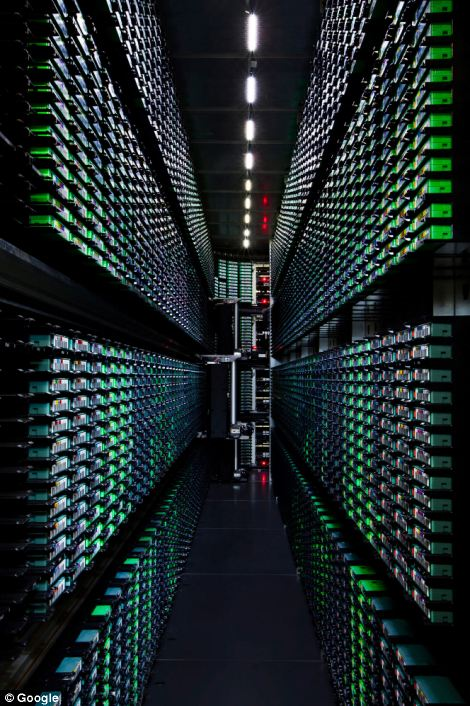
\includegraphics[trim=0 0 0 -20mm, width=\textwidth]{Images/computing}
		\end{column}}
	\end{columns}
\end{frame}

\begin{frame}{Fidelity on Product Graphs}
	\begin{align*}
		f^{G\times H}_{N\times N'}(t) &= \left( \bra{N} \otimes \bra{N'} \right)e^{-\text{i}A_{G\times H}t} \left( \ket{1} \otimes \ket{1'} \right) \\
		&= \left( \bra{N} \otimes \bra{N'} \right)e^{-\text{i}(A_G \otimes \text{1}_{V_H})t} e^{(\text{1}_{V_G} \otimes A_H)t} \left( \ket{1} \otimes \ket{1'} \right) \\
		&= \sum_{k=1}^{K}\left[ \left( \bra{N} \otimes \bra{N'} \right) \ket{g'_k}\bra{g'_k}e^{-\text{i}G_k{}'t} \ket{h'}\bra{h'}e^{-\text{i}H_k{}'t} \left( \ket{1} \otimes \ket{1'} \right) \right]
	\end{align*}
	\begin{itemize}
		\item $K = (V_{G\times H})$, $L = (V_G)$, $M = (V_H) \rightarrow K = L\cdot M$
		\item $\bra{g'_k} = \bra{g_l} \otimes \bra{e_m}$, $\bra{h'_k} = \bra{e_l} \otimes \bra{h_m}$ etc.
		\item $G_k{}' = G_l\cdot E_m$, $H_k{}' = E_l\cdot H_m$
		\item $(A\otimes B)(C\otimes D) = (AC)\otimes (BD)$
	\end{itemize}
	\begin{align*}
		f^{G\times H}_{N\times N'}(t) &= \sum_{l=1}^L\left[ \Braket{N|g}\Braket{g|1}e^{-\text{i}Gt} \right] \sum_{m=1}^M\left[ \Braket{N'|h}\Braket{h|1'}e^{-\text{i}Ht} \right] \\
		&= \Braket{N|e^{-\text{i}A_G t}|1}\Braket{N'|e^{-\text{i}A_H t}|1'}
	\end{align*}
\end{frame}

\begin{frame}[t]{Fidelity on Product Graphs}
	\begin{exampleblock}{}
	\setlength\abovedisplayskip{-8pt}
	\begin{center}
		$ f^{G\times H}_{N\times N'}(t) = f^G_N(t)\cdot f^H_{N'}(t) $
	\end{center}
	\end{exampleblock}
	\begin{align*}
		f^G_N(t) &= 1 \text{ for } t = t_G \\ 
		f^H_{N'}(t) &= 1 \text{ for } t = t_H \\ 
		f^{G\times H}_{N\times N'}(t) &= 1 \text{ for } t = t_{G\times H}
	\end{align*}
	\begin{exampleblock}{}
	\setlength\abovedisplayskip{-8pt}
	\begin{center}
		$ \text{iff }\frac{t_G}{t_H} \in \mathbb{Q} \rightarrow t_{G\times H} = LCM(t_G,t_H) $
	\end{center}
	\end{exampleblock}
\end{frame}

\section{Examples}
\subsection{Spin Chains}
\begin{frame}{Spin Chains}

%    PST, max 3, sketch of proof, fidelity
\end{frame}

\subsection{Spin Networks}
\begin{frame}[t]{Cartesian Product of Graphs}
    Spin chains too short -> more complex networks, explain kronecker product of graphs, sketch proof for fidelity decomposition, hypercubes, flattened versions.
\end{frame}

\subsection{Spin Switch}
\begin{frame}{Local Potentials}
    Pic of Switch, Variety low, introduce local potentials, only affect diagonal entries, add loops to vertices (left out for clarity), realized as magnetic fields etc.
\end{frame}

\begin{frame}{Spin Switch}
    sketch calculation, more arms handled by renormalization, fidelities
\end{frame}

\subsection{Switch$^2$}
\begin{frame}{Switch$^2$}
    graph product works with local potentials as well, added at each site, symmetries, more arms.
\end{frame}

\section{Roadmap}
\subsection{Varying Couplings}
\begin{frame}{Varying Couplings}
    Local couplings leads to much more variety, spin chains with perfect couplings (isomorphism of hilbert spaces to spin n-something particle), not yet looked at switch
\end{frame}

\subsection{Higher Excitation Subspaces}
\begin{frame}{Higher Excitation Subspaces}
    Possibility to control more than one qubit at each site, rings, QEC and fault tolerance, easy to calculate higher spin subspace graphs and hamiltonians, even full hamiltonian
\end{frame}

\subsection{Entanglement}
\begin{frame}{Entanglement}
    Dynamics of entanglement, teleportation for transport.
\end{frame}

\subsection{Experimental Verification}
\begin{frame}{Experimental Verification}
    Some experiments verify these results, Georgios paper (cm4) for two-spin up subspace analysis and great pictures, quantum dots
\end{frame}

\section{Goal}
\begin{frame}{Goal}
    Define general constraints on hamiltonians so that the single spin subspace graph leads to a network automatically capable of perfect state transfer, hints: symmetry, EV difference quotient rational, connectivity.
\end{frame}

\end{document}
